\documentclass[5p,times,twocolumn,10pt]{elsarticle}
%%%%%%%%%%%%%%%%%%%%%%%%%%%%%%%%%%%
\usepackage{graphicx} % allows inclusion of graphics
\usepackage{booktabs} % nice rules (thick lines) for tables
\usepackage{tabulary}
\usepackage{microtype} % improves typography for PDF
\usepackage{xcolor}
\usepackage{amsmath}
\usepackage{bm}
\usepackage{tikz}
\usepackage{verbatim}
\usepackage[superscript,nospace]{cite}
\usepackage{amssymb}
\usepackage[amssymb,cdot]{SIunits}
\usepackage{standalone}
\usepackage{subcaption}
%%%%%%%%%%%%%%%%%%%%%%%%%%%%%%%%%%%
% put your own definitions here:
\newcommand{\SN}{S$_N$}
\renewcommand{\vec}[1]{\bm{#1}} %vector is bold italic
\newcommand{\vd}{\bm{\cdot}} % slightly bold vector dot
\newcommand{\grad}{\vec{\nabla}} % gradient
\newcommand{\ud}{\mathop{}\!\mathrm{d}} % upright derivative symbol
\newcommand{\oper}[1]{\mathcal{#1}}
\providecommand{\e}[1]{\ensuremath{\times 10^{#1}}}
\newcommand{\CHAPTER}[1]{Chapter~\ref{#1}} 
\newcommand{\EQ}[1]{Eq.~(\ref{#1})}               %-- Eq. (refeq)
\newcommand{\EQUATION}[1]{Equation~(\ref{#1})}    %-- Equation (refeq)
\newcommand{\FIG}[1]{Fig.~\ref{#1}}               %-- Fig. refig
\newcommand{\FIGS}[2]{Fig.~\ref{#1}~and~\ref{#2}} %-- Fig. refig
\newcommand{\FIGURE}[1]{Figure~\ref{#1}} 
\newcommand{\TAB}[1]{Table~\ref{#1}}              %-- Table tablref
\newcommand{\EQS}[2]{Eqs.~(\ref{#1})--(\ref{#2})}            %-- Eqs. (refeqs)
\newcommand{\EQUATIONS}[2]{Equations~(\ref{#1})--(\ref{#2})}   %-- Eqs. (refeqs)
\newcommand{\EQSTWO}[2]{Eqs.~(\ref{#1})~and~(\ref{#2})}     %-- Eqs. (refeqs)
\newcommand{\EQUATIONSTWO}[2]{Equations~(\ref{#1})~and~(\ref{#2})} 
%-- Eqs. (refeqs
\newcommand{\BOXEQ}[1]{\mbox{\fboxsep=.13in $$
        \framebox{$ #1 $} $$ } }    %-- box around equation
\newcommand{\REF}[1]{Ref.~\citen{#1}}
\DeclareMathOperator*{\dotp}{{\scriptscriptstyle \stackrel{\bullet}{{}}}}
%%%%%%%%%%%%%%%%%%%%%%%%%%%%%%%%%%%
\begin{document} 
%%%%%%%%%%%%%%%%%%%%%%%%%%%%%%%%%%%
\begin{frontmatter}

%% Title, authors and addresses

\title{Application of the Karhunen-Lo\`{e}ve Transform to the C5G7 benchmark in 
the Response Matrix Method}

\author{Richard L. Reed}
\ead{rlreed@k-state.edu}
\author{Jeremy A. Roberts\corref{cor1}}
\cortext[cor1]{Phone number: 785-532-7182}
\ead{jaroberts@k-state.edu}

\address{
Mechanical and Nuclear Engineering, Kansas State University, Manhattan, KS
}

% \ead{rlreed@k-state.edu \and jaroberts@k-state.edu}

\begin{abstract}
Presented is an application of the Karhunen-Lo\'eve Transform (KLT) for treatment of the energy variable in response matrix methods  to a 44-group version of the the 2-D C5G7 benchmark problem.  Response matrix methods are based on the partitioning of global domains into independent nodes linked by boundary conditions approximated by truncated expansions of the phase space in orthogonal bases.  Here, KLT was used to produce basis sets appropriate for the energy variable based on ``snapshots.''  The method of snapshots employs small, representative problems to provide input spectra with which the KLT produces an orthogonal basis for the application. For this study, several computationally small models were defined, and the success of the corresponding basis was compared to the  reference (full-multigroup) solution.  The best performing basis sets were generated using information from both the scalar flux and the partial current, and typically included information from each unique material (e.g., a UO\textsubscript{2} pin cell) in the application problem and junctions between such materials (e.g., a UO\textsubscript{2} adjacent to a MOX pin cell).  In general, the KLT performed better than the standard discrete Legendre Polynomials (DLPs) as well as ``modified'' DLPs with proper snapshot selection.  The largest errors were found at the material junctions, precisely where spectral gradients are greatest.
\end{abstract}

\begin{keyword}
Basis Generation \sep Expansion in Energy \sep Response Matrix Method \sep Karhunen-Lo\'eve Transform
%% keywords here, in the form: keyword \sep keyword

%% MSC codes here, in the form: \MSC code \sep code
%% or \MSC[2008] code \sep code (2000 is the default)

\end{keyword}

\end{frontmatter}
%%%%%%%%%%%%%%%%%%%%%%%%%%%%%%%%%%%
\section{Introduction}

Previous work used the Karhunen-Lo\`{e}ve Transform (KLT) to create
basis sets for representing the energy variable in the eigenvalue response 
matrix method (ERMM) and demonstrated the efficiency of such basis sets for 
1-D problems \cite{annualANS, reedThesis, reed2015energy}. 
 The present work provides an extension of the KLT basis sets to a modified version of
 the 2-D, C5G7 benchmark problem building from previous results \cite{winterANS}. ERMM solves the reactor eigenvalue equation,
\begin{equation}
  \mathcal{T} \phi(\bm{\rho}) = 
    \frac{1}{k} \mathcal{F} \phi(\bm{\rho}) \, ,
  \label{eq:global}
\end{equation}
where $\bm{\rho}$ contains the relevant phase space (i.e., space, angle, and 
energy),
by decomposing the domain into independent nodes linked through approximate  
boundary conditions that are based on truncated, orthogonal basis expansions.  
The 
success of ERMM in realistic applications is highly dependent on the 
selection of orthogonal bases in each phase space variable.  Basis 
sets that capture 
high-fidelity transport solutions with low-order expansions are ideal. 

The goal of this work was to test the applicability of the method of snapshots and 
the KLT to 2-D problems.  The C5G7 benchmark was adapted to use a 44-group 
cross-section library, which greatly increases the size of the problem, and 
thus the computation time.  In what follows, ERMM and KLT basis are briefly 
reviewed, and their application 
to a modified C5G7 problem is presented.

%%%%%%%%%%%%%%%%%%%%%%%%%%%%%%%%%%%
\section{Methods}
%%%%%%%%%%%%%%%%%%%%%%%%%%%%%%%%%%%
\subsection{Overview of ERMM}

Suppose the global problem of \EQ{eq:global} is defined over a 
volume $V$ which can be decomposed into $N$ disjoint, nodal subvolumes
$V_i$ that satisfy $V = V_1 \bigcup V_2 \bigcup \ldots \bigcup V_N$.
Then a local transport problem for the $i$th node is defined
\begin{equation}
  \mathcal{T} \phi(\bm{\rho}_i) = 
    \frac{1}{k} \mathcal{F} \phi(\bm{\rho}_i) \, ,
  \label{eq:local}
\end{equation}
subject to the incident current boundary condition
\begin{equation}
  J^{\mathrm{}}_{-} (\bm{\rho}_{is}) = 
    J^{\mathrm{global}}_{-}(\bm{\rho}_{is}) \, ,
  \label{eq:localbc}
\end{equation}   
where $J_{-} (\bm{\rho}_{is}) $ is the incident angular current on 
surface $s$.  To reduce the size of the problem space, the local boundary 
currents are represented as a truncated 
expansion in an 
orthogonal basis, $P_m(\bm{\rho}_{is}), \,\,\, m = 0, \, 1, \, \ldots$,
defined over the surface phase space $\bm{\rho}_{is}$.
By solving \EQ{eq:local} subject to the $m$th order 
incident condition
\begin{equation}
 J_{-} (\bm{\rho}_{is}) = P_m(\bm{\rho}_{is}) \, 
\end{equation}
on one surface, $s$, and vacuum elsewhere, 
a response function is defined as
\begin{equation}
       r^{ms}_{im's'} = \int d\rho_{is'} P_{m'}(\bm{\rho}_{is'})  
        J_{+} (\bm{\rho}_{is'}) \, ,
\label{eq:responsefunction}
\end{equation}
where $J_+$ is the outgoing angular current.  The 
response function $r^{ms}_{im's'}$ 
is the $m'$th order current response out of 
surface $s'$ due to an $m$th order incident current on 
surface $s$.

By expressing the incident and outgoing currents, $J_{\mp}$, as truncated  
expansions in the basis, global neutron balance can be represented by the 
response matrix equation 
\begin{equation}
  \mathbf{M}\mathbf{R}(k)\mathbf{J_-}  = \lambda \mathbf{J_-} \, ,
\label{eq:erme}
\end{equation}
where $\mathbf{R}$ contains response functions, $\mathbf{J}_{-}$ contains the  
incident angular current expansion coefficients, $\mathbf{M}$ is a matrix that 
redirects outgoing currents as incident currents of neighbors, and $\lambda$ is 
an eigenvalue that approaches unity as $k$ approaches its correct value. The 
$k$-eigenvalue is computed iteratively by alternately solving for 
$\mathbf{J}_{-}$ and updating $k$ based on balance \cite{RobertsSerment}.
%%%%%%%%%%%%%%%%%%%%%%%%%%%%%%%%%%%
\subsection{Expanding in Energy}

The present work focused solely on expansion of the energy variable.  
Traditionally, RMMs have used a full multigroup 
representation of the energy variable, which is to say no truncation for 
the energy basis is used.  Response matrix methods have been used 
successfully with a variety of energy group structures, ranging from three to 
190 groups \cite{ishii2009tdd, forget2006tdh, forget2004hcm}. 

In general, response methods are prohibitively expensive unless the problem space is 
greatly reduced by truncating the boundary conditions of each node.  Thus, an 
effective basis set will permit the use of a low-order expansion without 
introducing a large error.  Realistic problems require on the order of dozens 
of energy groups 
or more, and a basis that can capture many-group fidelity with 
many fewer energy degrees of freedom would be of substantial 
value to RMM.  

Recent work investigated the use of discrete Legendre polynomials (DLP) and  
modified DLP (mDLP) for expansion in energy \cite{Roberts2014}.  The mDLP basis 
modifies the DLP basis by superimposing a ``shape'' vector on each basis vector. 
 The shape vector is chosen to be representative of the vector subject to 
expansion, i.e., the energy-dependent angular current.  Previously, a spatially 
averaged energy spectrum from a representative lattice problem has been used 
with moderate success \cite{Roberts2014}.

%%%%%%%%%%%%%%%%%%%%%%%%%%%%%%%%%%%
\subsection{The  Karhunen-Lo\`{e}ve Energy Basis}

A more powerful approach (compared to mDLP) of incorporating physics into the 
basis functions is to use the Karhunen-Lo\`{e}ve transform (KLT)
\cite{Dony2001}.  The central goal of KLT is to approximate a discrete or 
continuous function $f(x)$ as a truncated expansion in an orthogonal basis whose 
functions yield the best possible $n$th-order approximation in terms of 
least-squares error for all values of $n$ by extracting information about the 
representative spectra in the problem space.  In some applications, such as 
image compression, the function $f$ is predetermined, e.g., a set of pixel 
values, while in other applications, such as reduced-order modeling, the 
function $f$ is not known.  While details of its use in these applications may 
differ, KLT is fundamentally related to the singular value decomposition (SVD) 
\cite{reedThesis}.

The implementation algorithm for computing the basis 
functions, $P^i_{\text{KLT}}(:)$, begins by forming the data matrix 
$\mathbf{D}$.  Let the $n$th current vector be denoted by 
$\mathbf{d}_n$.  These 
vectors, referred to as snapshots, are combined to form the 
matrix $\mathbf{D} \in \mathbb{R}^{G\times N}$, which is defined as $\mathbf{D} 
= [\mathbf{d}_1,\, \mathbf{d}_2,\, \ldots, \, \mathbf{d}_N]$  
\cite{Meyer2002}, where $G$ is the number of energy groups and $N$ is the total
number of snapshots. Then the matrix 
$\mathbf{B} \in \mathbb{R}^{N\times N}$ is defined as
\begin{equation}
    \mathbf{B} = \mathbf{D}^{\intercal}\mathbf{D} \, .
    \label{eq:KLT}
\end{equation}
Next, find the eigenvectors corresponding to the largest eigenvalues of the 
matrix 
$\mathbf{B}$,
\begin{equation}
    \label{eq:SVD_of_B}
    \mathbf{B} = \mathbf{Q}\mathbf{\Lambda}\mathbf{Q}^{-1}\, ,
\end{equation}
where $\mathbf{Q}$ from \EQ{eq:SVD_of_B} is equal 
to $\mathbf{V}$ 
from the SVD of $\mathbf{D}$, and is thus the set of 
eigenvectors of 
$\mathbf{D}$. The eigenvectors $\mathbf{q}_j$ (columns of $\mathbf{Q}$ from 
\EQ{eq:SVD_of_B}), are 
then multiplied by the data matrix to form the basis vectors $P^j_{KLT}(:)$, 
i.e.,
\begin{equation}
    P^j_{KLT}(:) = \mathbf{D}\mathbf{q}_j \, ,
\end{equation}
which are subsequently orthonormalized.  Then, an approximate representation of 
an arbitrary $N$-vector $\mathbf{f}$ in the basis is 
\begin{equation}
    \mathbf{f} \approx \sum_j a_j P^j_{KLT}(:) \, \quad \text{where} \quad a_j 
    = 
    \mathbf{f}^T P^j_{KLT}(:) \, .
    \label{eq:KLT_def}
\end{equation}

Since KLT requires information about the solution {\it a priori}, small models 
that are similar to the test problem are developed to provide the necessary 
information.  This work identifies how similar the small models need be to 
provide an adequate representation of the test problem. KLT snapshots are 
energy group-dependent flux or current vectors from several spatial cells within 
one or more representative models. 
%%%%%%%%%%%%%%%%%%%%%%%%%%%%%%%%%%%
\subsection{Test Problem}

To test the application of KLT in 2-D space, the C5G7 benchmark problem was 
adapted for use.  This benchmark consists of a 
quarter core that has four, $17\times17$-pin 
assemblies \cite{C5G7}.  The configuration is detailed in  
\FIG{fig:C5G7_config}.  Each of the blocks in \FIG{fig:C5G7_config} 
represent either a fuel assembly or an equivalent area of 
moderator.  Each pincell is broken up into a $7\times7$ 
Cartesian mesh. Thus, each pincell contained 49 spatial cells and provided 49 
energy dependent snapshots of each type (scalar flux, partial current, etc.).  
The cladding for the pincells was 
homogenized into the fuel part of the pincell.  

The standard C5G7 benchmark uses seven-group cross-sections, which precludes 
the need for an energy approximation.  Thus, a cross-section library was 
generated with SCALE 5.1 in the SCALE 44-group format \cite{Scale}.  All other 
aspects of the benchmark were unchanged.

\begin{figure}[htb]
    \centering
    \includestandalone[mode=buildnew]{figures/c5g7}
    \caption{Configuration for C5G7 benchmark.  Each square represents the area 
of a 
             $17\times17$ pin assembly}
    \label{fig:C5G7_config}
\end{figure}

To complete this work, the ERMM solver SERMENT \cite{RobertsSerment} was used
for all calculations.  The program expands each of the phase space variables
to a given order using a given basis set.  The expansion order for the reference solution and the RMM
solutions for each 
snapshot case were set to fourth order in space and angle. It is assumed that the relative 
error of the snapshot cases is a function of the energy expansion alone since 
all other aspects of the problem are identical between the reference solution 
and each test case.  It is impossible to be sure whether this assumption is valid 
with the available resources without computing the problem at higher order.
%%%%%%%%%%%%%%%%%%%%%%%%%%%%%%%%%%%
\subsection{Generation of Snapshots}

\begin{table*}[htb]
    \centering
    \caption{Summary of snapshot models for C5G7 test Problem}
    \begin{tabulary}{\linewidth}{c | L}\toprule
        Abbreviation         & Model to generate snapshots \\ \midrule
        Reduced Full-Core    & Spatially-averaged snapshots from whole core 
model (i.e.,         the test problem) \\
        Combined-Assemblies  & Snapshots from assemblies used in core 
                               configuration \\
        Combined-Pins        & Snapshots from pins used in core 
                               configuration combined with the pin 
                               junctions\\
        Small-Core           & Snapshots from the small core model \\
        Small-Assemblies     & Snapshots from the small assemblies used in the 
                               small core configuration \\
        Reduced Small-Core   & Spatially-averaged snapshots from the small core 
model \\
        1-D Approximation    & Snapshots from the 1-D approximation to the C5G7 
                               benchmark \\
        \bottomrule
    \end{tabulary}
    \label{tab:C5G7snapshots}
\end{table*}

There are several models that are readily apparent choices to simplify the C5G7 
benchmark for use in generating snapshots.  The snapshots models used for 
this test problem are summarized in \TAB{tab:C5G7snapshots}.  The first model 
was to use snapshots from the test problem itself to gain an understanding of 
the best possible snapshots.  However, the number of snapshots obtained for this 
model is prohibitively large, even after removing all duplicate snapshots by 
model symmetry, and thus the model was unusable in the raw state.  However, by spatially 
averaging the snapshots over a pincell, the number of 
snapshots is reduced by a factor of 49, and leads to a manageable set of functions with 
which to create a basis; this model is referred to as the Reduced Full-Core model. 

The Combined-Assemblies model was formed by modeling a UO$_2$ assembly with reflective 
boundary conditions, extracting snapshots, and combining the snapshots together
with those from a similarly processed MOX assembly.  

Similarly formed is the 
Combined-Pins model, which derives snapshots from individual pincells for each 
fuel type each modeled with reflective boundary conditions.  In this case, however, 
the pincell snapshots were combined with snapshots from junctions of 
pincells. These junctions were modeled as 
$2\times2$-pin assemblies with 
reflective conditions as shown in \FIG{fig:junction}.  There were a total of five different materials, thus 
ten unique junctions to model. The snapshots from the ten junctions and four 
fuel pincells were combined to form the Combined-Pins model.

\begin{figure}[htb]
    \centering
    \resizebox{0.45\columnwidth}{!}{
    \includestandalone[mode=buildnew]{figures/junction}}
    \caption{Configuration for pincell junction; all Reflect BC; Every 
        combination is used}
    \label{fig:junction}
\end{figure}

A sequence of models were generated by creating a small version of the C5G7 core, which 
has the same assembly configuration shown in \FIG{fig:C5G7_config}, but 
instead uses $8\times8$-pin assemblies \cite{reedThesis}, which is called
the Small-Core model.  An additional model 
arises from the small core, which is to form the Small-Assemblies model 
similarly to the Combined-Assemblies, but using $8\times8$-pin assemblies. 
While this was not expected to perform as well as the full-sized, 
Combined-Assemblies model, it was less expensive to create the snapshots, and 
thus the corresponding basis functions.  
A third model from the small core was to spatially 
average the snapshots over each pincell similarly to the Reduced Full-Core model.  This Reduced Small-Core model was used to approximate the 
non-spatially averaged, Full-Core model by comparing the reduced and non-reduced 
Small-Core models.  

The final snapshot model used for the C5G7 test problem was to create a 
similar 1-D model with three sections: UO$_2$, MOX, and 
moderator as shown in \FIG{fig:1d_config}.  The model is comprised of 51 pins that are each of width 1.26 cm.  
This problem was created with a reflective boundary condition on the UO$_2$ 
side of the model and a vacuum boundary condition on the moderator side of the 
model.

\begin{figure}[htb]
    \centering
    \resizebox{0.9\columnwidth}{!}{
    \includestandalone[mode=buildnew]{figures/1d}}
    \caption{Configuration for 1D approximation to the C5G7 benchmark.  The 
             green represents UO$_2$, the light red represents 
             4.3\% MOX fuel, the medium red represents 7.0 \% MOX fuel, and the 
             dark red represents 8.7\% MOX fuel, and the blue 
             represents moderator}
    \label{fig:1d_config}
\end{figure}

In general, snapshot models should
be computationally quick to solve, yet similar to the test problem.  Timing 
studies provide little insight in this study because the snapshots are orders of 
magnitude quicker to generate than the response matrices. Furthermore, it is 
impossible to know {\it a priori} how many basis functions are required for 
accuracy before generating the response matrices.

%%%%%%%%%%%%%%%%%%%%%%%%%%%%%%%%%%%
\section{Results and Analysis}
 
For brevity, the results for this section have been 
truncated from a full 43rd order expansion.  The overarching goal of the work was to achieve 
sub-$0.1\%$ relative pin 
power errors while reducing the necessary energy degrees of freedom by an order 
of magnitude.  As such, a model should reach the error goal by 9th order to successfully meet
the overarching goal in a 2-D problem-space.

\begin{figure}[htb]
\resizebox{0.9\columnwidth}{!}{
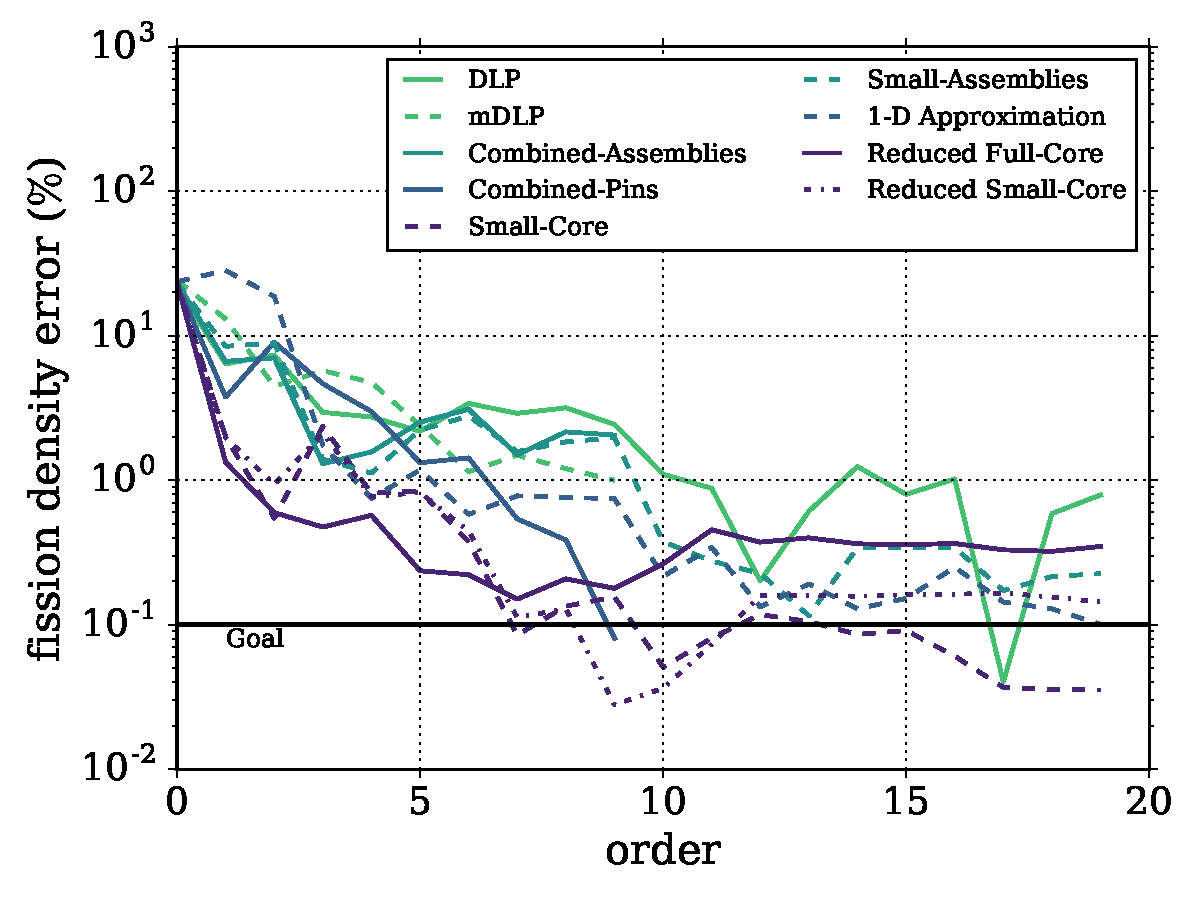
\includegraphics[trim=.1cm .25cm 2.0cm .4cm clip=true, 
]{figures/energy_basis_comparison_fission-20}}
\caption{Maximum relative error in fission density for 44-group, C5G7 test problem using snapshot of only $\phi$.}
\label{fig:c5g7-flux-only}
\end{figure}

\begin{figure}[htb]
\resizebox{0.9\columnwidth}{!}{
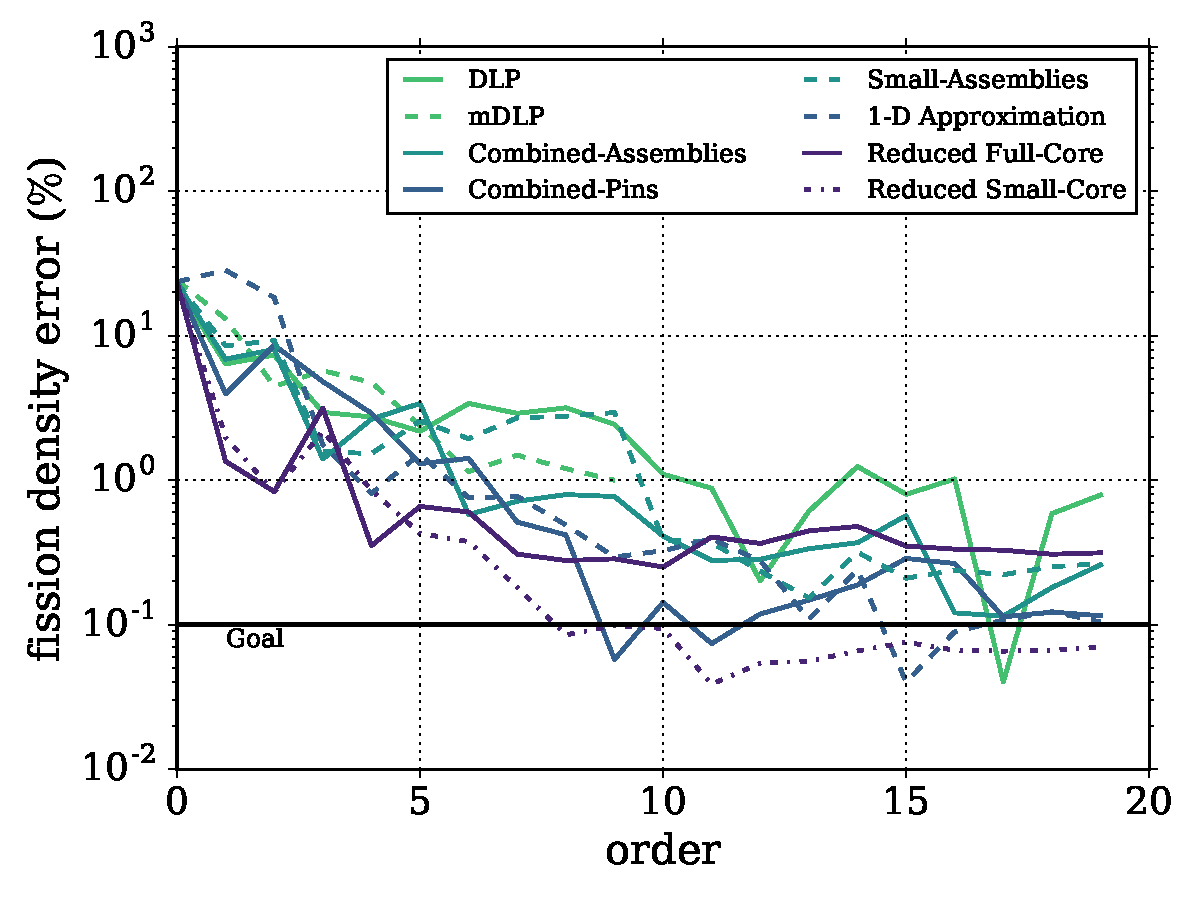
\includegraphics[trim=.1cm .25cm 2.0cm .4cm clip=true, 
]{figures/partial_energy_basis_comparison_fission-20}}
\caption{Maximum relative error in fission density for 44-group, C5G7 test problem using snapshot of $\phi$, $J_{\text{up}}$, and $J_{\text{down}}$.}
\label{fig:c5g7-combined}
\end{figure}

\begin{figure}[htb]
\resizebox{0.9\columnwidth}{!}{
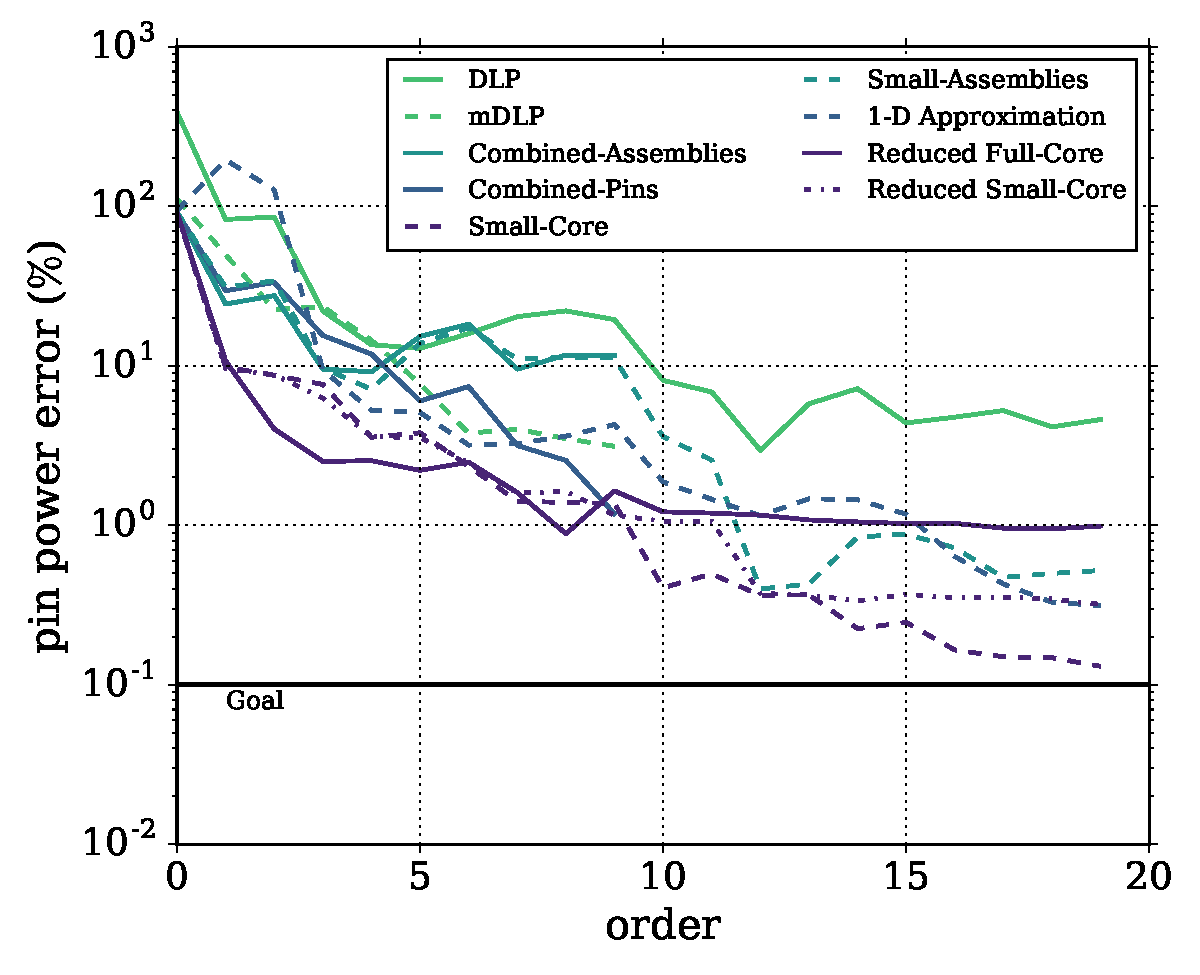
\includegraphics[trim=.1cm .25cm 2.0cm .4cm clip=true, 
]{figures/energy_basis_comparison_pinpower-20}}
\caption{Maximum relative error in pin power for 44-group, C5G7 test problem using snapshot of only $\phi$.}
\label{fig:c5g7-flux-only-pp}
\end{figure}

\begin{figure}[htb]
\resizebox{0.9\columnwidth}{!}{
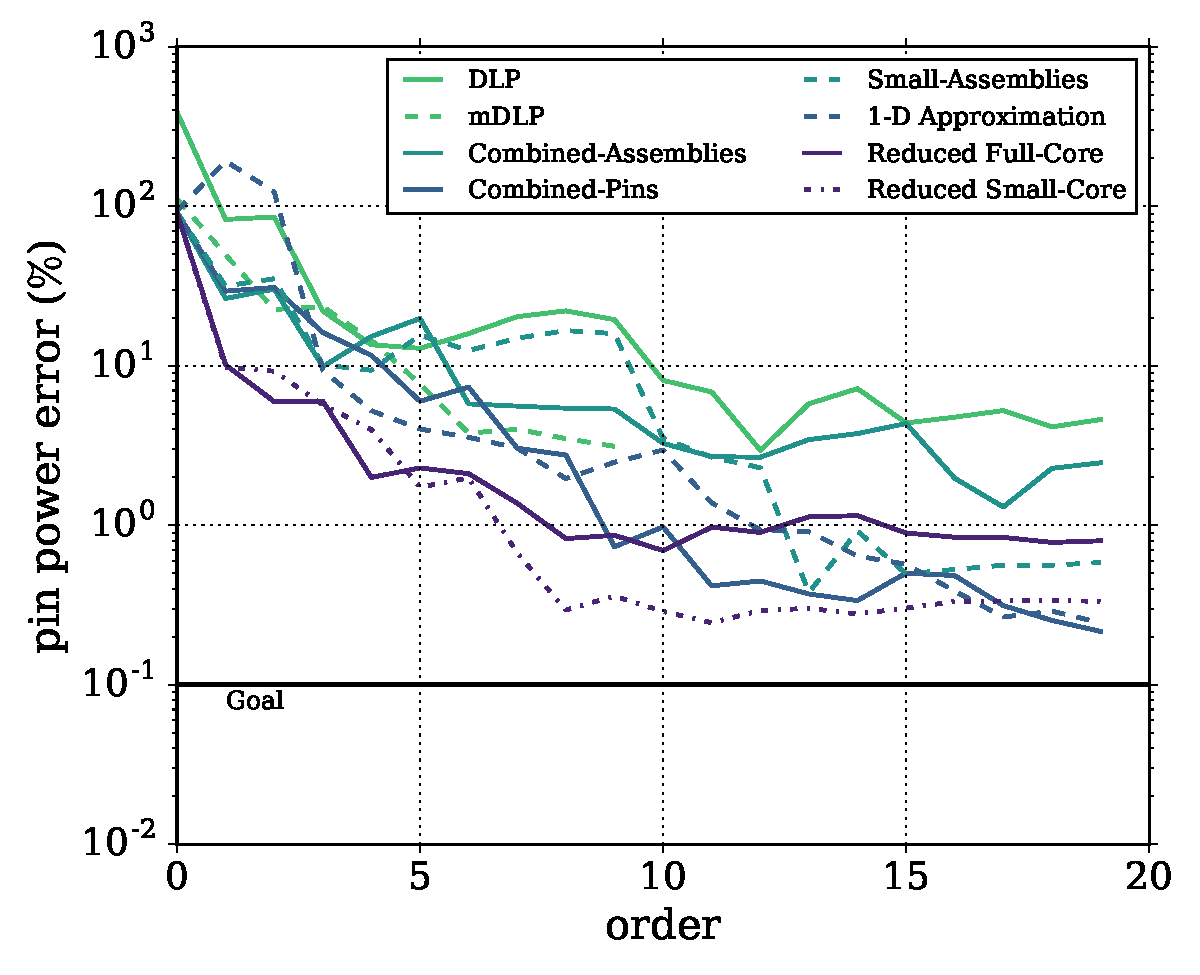
\includegraphics[trim=.1cm .25cm 2.0cm .4cm clip=true, 
]{figures/partial_energy_basis_comparison_pinpower-20}}
\caption{Maximum relative error in pin power for 44-group, C5G7 test problem using snapshot of $\phi$, $J_{\text{up}}$, and $J_{\text{down}}$.}
\label{fig:c5g7-combined-pp}
\end{figure}

Each curve shown in this section except for `DLP' and `mDLP' was 
generated using the KLT basis with distinct snapshot data. The mDLP results 
represent the best method previously observed \cite{roberts2014psb}, i.e., the 
mDLP shape vector (flux spectrum for the C5G7 problem with 44 energy groups)
was applied to each DLP vector.  
\FIGURE{fig:c5g7-flux-only} presents the results from using snapshots of only 
the scalar flux $\phi$ in the KLT basis generation in order to approximate the 
nodal fission densities.  

As a first basis for comparison, the maximum relative error of the nodal fission density
was compared for a snapshot 
model.  The nodal fission density is almost equivalent to the assembly power, 
and the reference is taken to the be nodal fission density from a full 
multigroup solution of the modified C5G7 problem using the 44-group cross-section 
library. 

First, the results of utilizing snapshots of only the scalar flux 
$\phi$ to generate the KLT basis functions are presented in 
\FIG{fig:c5g7-flux-only}, where the maximum relative error of the 
nodal fission density is shown as a function of energy degree of freedom.  
By nine degrees of freedom, none of the models consistently reached the goal of 
sub-$0.1\%$ errors; however, several models performed well.  The 
Small-Core model performed well despite spatially reducing the problem by a factor 
of four.  Surprisingly, one of the best performing models was the Combined-Pins model despite its 
simplicity. Both of these snapshot models outperformed mDLP and 
reached nodal fission errors of sub-$1\%$ by at least 7th order.  
As \FIG{fig:c5g7-flux-only} shows, the results of the Small-Core and 
Reduced Small-Core were quite similar, with the Small-Core results performing 
slightly better in terms of the maximum relative error.  Based on this 
similarity, the Reduced Full-Core results were assumed
approximately equal to the Full-Core results, and thus are used as a 
surrogate for the best possible basis set for application to the C5G7 problem.

In the 2-D case, the partial current $J$ cannot be assumed symmetric in all directions,
thus the partial currents in the up and down directions were chosen.  
Due to the symmetry of the C5G7 model, the partial currents in the up and down
direction are equivalent to partial currents in the left and right directions,
thus the choice was made arbitrarily.  
\FIGURE{fig:c5g7-combined} presents the results from using snapshots from 
$\phi$, $J_{\text{up}}$, and $J_{\text{down}}$.  The inclusion of the 
partial currents had varying effects on the performance of each snapshot model, e.g., the Reduced 
Small-Core model was improved in general, while the Small-Assemblies model was worsened.  The 
Combined-Pins results were relatively unchanged. However, the best performing basis sets in general were those that included 
the information of the partial current and the scalar flux.

For an additional comparison, the maximum relative error 
in the pin powers were compared for each of the snapshot models.  The reference 
case for this comparison was taken as the pin powers from a full multigroup 
solution of the C5G7 problem using the 44-group cross-section 
library.  It was expected that the pin power results would be inferior to the 
nodal fission density results because resolving the pin powers is more difficult 
than resolving the nodal fission density.  Thus, more energy degrees of freedom 
are required to achieve the same level of accuracy in general. 

\FIGURE{fig:c5g7-flux-only-pp} shows the results utilizing snapshots of only the 
scalar flux $\phi$, and as expected, the results were approximately an order of 
magnitude worse than the equivalent results solving for the fission density.  
However, the snapshot models appeared to perform consistently relative to 
each other.  The best performing case was the Reduced Small-Core, while the 1-D 
Approximation also performed well.  Also note that the Reduced Small-Core 
results were nearly identical to the Small-Core results, which suggests that the 
Reduced Full-Core results would have been nearly equivalent to the Full-Core results.  
However, more energy degrees of freedom were needed to resolve the pin powers to 
the desired accuracy.

When combining snapshots of $\phi$, $J_{\text{up}}$, and $J_{\text{down}}$, the relative 
error in pin power resolution was slightly improved as \FIG{fig:c5g7-combined-pp} shows.  The 
Small-Core model reached sub-$1\%$ relative 
error by approximately seventh order, assuming that the error did not increase 
in the higher orders.  When using all available snapshots, most 
cases performed better than using only one type of snapshot alone.

The error in the pin powers of the best performing KLT case (9th order 
Reduced Small-Core) using only $\phi$ snapshots relative to the SERMENT 
reference solution is presented as a heat map in \FIG{fig:serklt}.  In this 
figure, the maximum error is located at the center of the figure as well as the MOX junctions.

\begin{figure}[htb]
\resizebox{0.9\columnwidth}{!}{
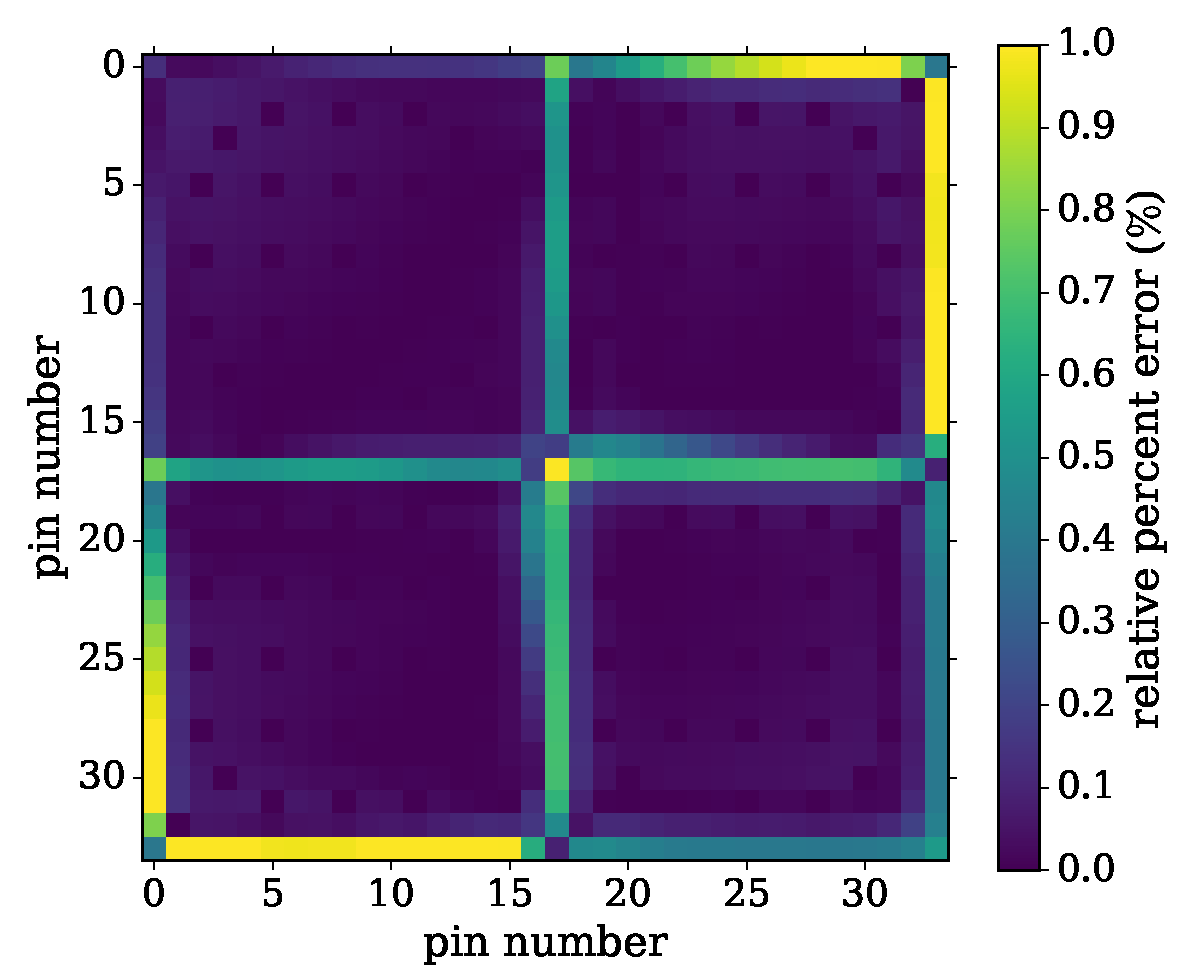
\includegraphics[trim=.1cm .25cm 2.0cm .4cm clip=true, 
]{figures/serklt8_error}}
\caption{Error in the pin powers of the best performing KLT case (9th 
order, Reduced Small-Core) relative to the SERMENT 
reference solution using snapshots of $\phi$ only}
\label{fig:serklt}
\end{figure}

\begin{figure}[htb]
\resizebox{0.9\columnwidth}{!}{
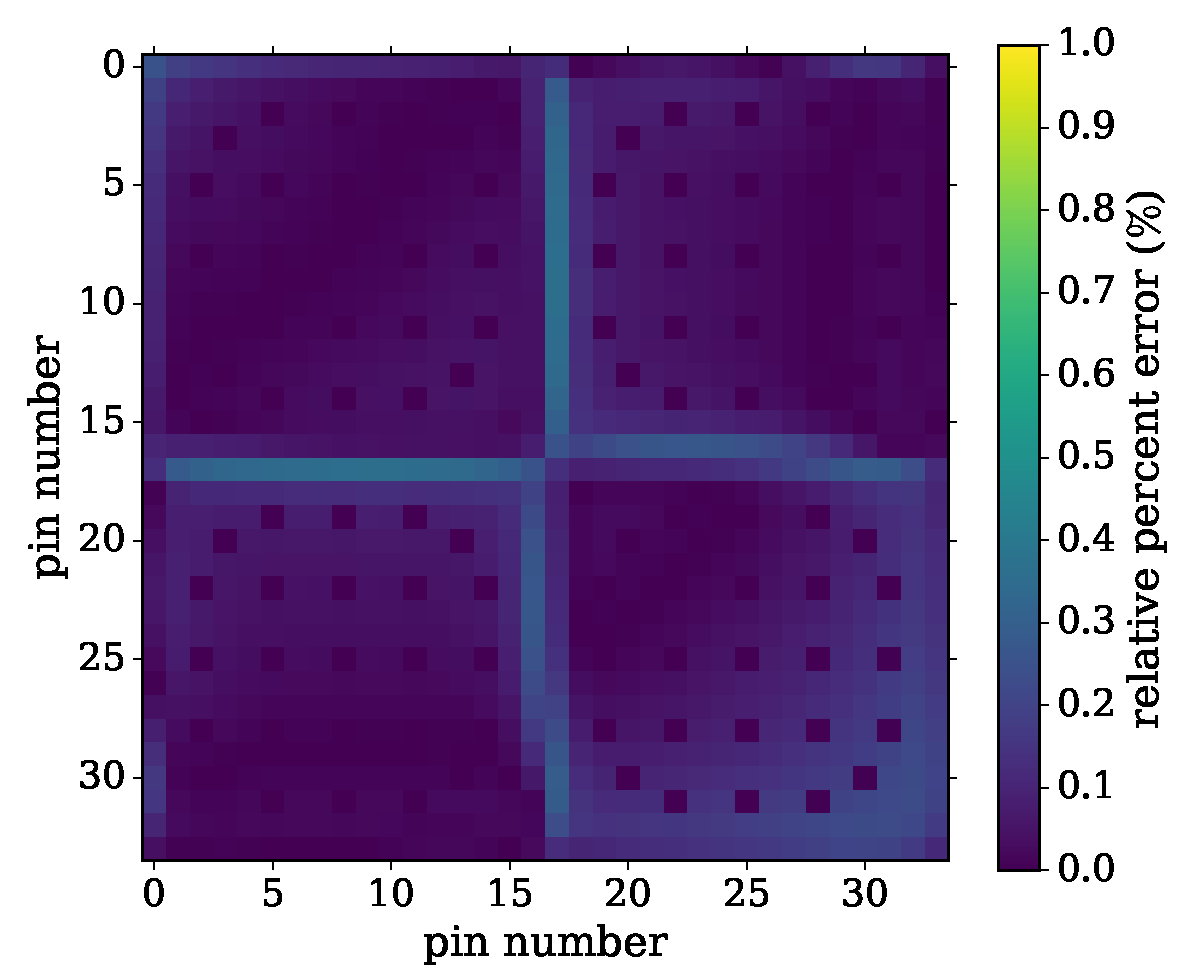
\includegraphics[trim=.1cm .25cm 2.0cm .4cm clip=true, 
]{figures/partial_serklt8_error}}
\caption{Error in the pin powers of the best performing KLT case (9th 
order, Reduced Small-Core) relative to the SERMENT 
reference solution using snapshots of $\phi$, $J_{up}$, and $J_{down}$}
\label{fig:serkltpartial}
\end{figure}

Finally, the error of the best performing KLT case from using $J_{up}$ and $J_{down}$ snapshots 
and $\phi$ snapshots (9th order, Reduced Small-Core) is presented in 
\FIG{fig:serkltpartial}.  When including partial-current information, the material
junctions were better captured, and the relative error was reduced.  The maximum error shown in 
\FIG{fig:serkltpartial} is located at the top, left cell of the figure, i.e., by the reflective boundary 
conditions at the center of the
model.

%%%%%%%%%%%%%%%%%%%%%%%%%%%%%%%%%%%
\section{Conclusion}

For 2-D problems, many KLT basis outperformed the mDLP and DLP bases for ERMM 
energy expansions because the KLT maximizes the information contained in 
low-order expansions.  In general, the results are 
improved by including the partial current in generation of snapshots as 
opposed to using only the scalar flux snapshots.  Including more relevant information
for KLT basis generation improves the applicability of the basis.

An effective snapshot model is one that can capture the relevant physics of 
the problem while remaining computationally inexpensive.  
In general, it seems that the size of the snapshot model is not a strong 
predictor of the success of a basis set, as the Combined-Pins model performs 
surprisingly well despite the model simplicity, and in some cases was the best 
performing in terms of the smallest maximum error at order nine.
The Combined-Pins likely succeeded because information 
about each fuel type as well as the junction between materials was used in 
the construction.  

The best performing basis functions were attained 
on average by including all available snapshots into basis generation.  However 
spatially averaging the snapshots did not appear to have a strong effect on 
the success of the basis set.  This was also expected because the snapshots 
provided by neighboring spatial cells were expected to be exceedingly similar.

The largest errors typically occurred at material and assembly junctions, which is 
expected, because the C5G7 benchmark was designed with difficult to capture junctions, 
to increase the difficulty of the benchmark.  It is interesting that including 
the partial current snapshots in basis generation improved the ability for capturing those junctions.  

It appears that for heterogeneous problems such as the C5G7 benchmark, a basis 
expansion in the energy variable requires more degrees of freedom to reach the 
goal of sub-0.1\% relative error as compared to the 1D problems previously 
explored \cite{annualANS, reedThesis}.  Future work in this area would entail 
expanding this application to additional group structures to explore any
group dependence of the results.  Additionally, it would be interesting to explore 
applications of the KLT to expansion in other phase space variables, e.g. space or angle.

%%%%%%%%%%%%%%%%%%%%%%%%%%%%%%%%%%%
\section{Acknowledgments}
The work of the first author was supported by the Kansas State University 
Nuclear Research Fellowship Program, generously sponsored by the U.S. Nuclear 
Regulatory Commission (Grant NRC-HQ-84-14-G-0033).

\section{References}
\bibliographystyle{elsarticle-num}
\bibliography{bibliography}
\end{document}